% !TeX root = ../main.tex
\chapter{Projection and Environmental Annotation}
\label{ch:data-environment}

The first module of our pipeline deals with the transformation and augmentation of our trajectories for the sake of locally accurate analysis:
Raw input trajectories usually use geodetic coordinates (lon/lat), which are not suitable for segmentation, kernel calculations, and random walk interpolations on a regular grid,
as these require metric coordinates.
For example, the shape and size of the area induced by 1° in longitude and latitude differs depending on the location on the globe.
Broadly speaking, there are three goals addressed by the several existing map projections, namely angle-, area- and length-preservation, which on a global scale stand in conflict with each other.
We aim to find a suitable projection of a trajectory's geodetic coordinates (EPSG:4326) to a regular grid for our dynamic program, and back to geodetic coordinates for visualization, that minimizes the 
errors induced by grid-discretization and distortion, caused by the earth's curvature.
Finally, the trajectories are augmented with terrain information, which can be used for the ensuing steps of our workflow, like segmentation and kernel calculations.

\section{Projection into a metric space}
For random-walk interpolation on a regular grid, a suitable projection should approximately satisfy the following conditions:
\begin{itemize}
  \item \textbf{Low distance distortion}: Equal grid increments should correspond to approximately equal distances on the Earth's surface. 
  Thus, grid cells should have a nearly constant ground size throughout the relevant area.
  \item \textbf{Conformality}: Local angles and changes in direction should be preserved, such that the shapes and directional properties of movement kernels are not distorted.
\end{itemize}

These requirements do not need to hold globally. In our pipeline, every animal is processed separately and its complete trajectory is reprojected independently. 
It is therefore sufficient that the projection introduces only small distortions over the area covered by the respective animal. 
The center and spatial extent of its trajectory can be used to select or define an appropriate local projection.

The resulting metric coordinates are used for segmentation, kernel generation, and grid-based random-walk interpolation. 
These steps are discussed in detail in Chapters~\ref{ch:segmentation}, \ref{ch:kernels}, and~\ref{ch:random-walks}, respectively. 
Geographic coordinates in EPSG:4326 are retained as the common input and output representation and are used for the final visualization of the results.

A natural initial choice for this per-animal projection is the Universal Transverse Mercator (UTM) system.

\subsection{Universal Transverse Mercator (UTM)}
The UTM coordinate system divides the Earth's surface between \(80^\circ\) South and \(84^\circ\) North into 60 longitudinal zones, each spanning \(6^\circ\) of longitude. 
The zones are numbered from 1 to 60 from west to east, starting at the \(180^\circ\) meridian. 
Each zone uses a separate transverse Mercator projection whose central meridian lies in the middle of the zone.
For identification, the UTM area is additionally divided into latitude bands. These are labelled from C to X from south to north, omitting the letters I and O. 
Most bands span \(8^\circ\) 
of latitude, while the northernmost band X spans \(12^\circ\). A zone number and latitude-band letter can be combined into a grid zone designation, such as 29U. 
The same zone numbers from 1 to 60 are repeated in every latitude band.

\paragraph{Properties: } UTM is based on the Transverse Mercator projection. Its projection cylinder is oriented along a selected zone's central meridian. 
For a zone with number $z$, its central meridian is 
\[\lambda_0 = 6z - 183^\circ\].
Each of the 60 zones defines an independent projected coordinate reference system (CRS). Therefore, coordinates from different UTM zones must not be combined directly. 
However, points outside a UTM zone can still be projected onto that zone's CRS, albeit with poorer projection properties. 
UTM is conformal, meaning that infinitesimally small shapes are preserved up to a scaling factor dependent on position. This is useful for movement directions, turning angles, and kernel shapes.
UTM uses metric coordinates, represented by eastings (E) and northings (N), which allow us to calculate a good approximation for the Euclidean distance directly. 
It uses a central scaling factor of $k_0$ = 0.9996, which causes distances along the central meridian to be slightly contracted. 
This scale factor increases with east-west distance from the central meridian and can be described approximately by the equation:
\[
k \approx k_0 \left( 1 + \frac{1}{2}(\Delta \lambda \cos \varphi)^2\right),
\]  
where $\Delta \lambda = \lambda - \lambda_0$ is calculated in radians. Consequently, UTM is neither distance- nor area-preserving, as distances are scaled by a factor of $k$ and areas by 
a factor of $k^2$, wherein $k$ increases quadratically with distance from the central meridian. 
However, these variations are usually small enough in practice, especially for the spatial extents and grid resolutions considered in this work.

A UTM CRS is specified by its zone number and hemisphere. The latitude-band letter is useful for identifying a geographic region, but is not part of the projected CRS itself. 
To avoid negative coordinate values, UTM uses a false easting of \(500\,000\,\mathrm{m}\). 
On the southern hemisphere, a false northing of \(10\,000\,000\,\mathrm{m}\) is additionally applied. 
Consequently, an easting and northing pair is only unambiguous when the corresponding zone and hemisphere are known.
For an example location in EPSG:4326 of 
\[
p = (\lambda, \varphi) = (7.1508^\circ\mathrm{E},51.2562^\circ\mathrm{N})
\]
the corresponding zone is calculated by \[
z
=
\left\lfloor
\frac{\lambda+180^\circ}{6^\circ}
\right\rfloor+1.
\]
The latitude of $p$ indicates that the point lies in the northern hemisphere ($\text{lat} \geq 0^\circ$). 
In these cases, the EPSG code equals $32600 + z$, otherwise ($\text{lat} < 0$) $32700 + z$.
Finally, $p$ is projected using EPSG:32632 to \[
(E,N)
=
(367\,366\,\mathrm{m},5\,677\,885\,\mathrm{m})
\]
, using established python libraries like PROJ.

\subsection{Local Transverse Mercator Projection}
In our workflow, we use a trajecory's center coordinate to determine the UTM zone and project every point of that trajectory to the
corresponding UTM CRS. This approach has two drawbacks. First, a trajectories center might be positioned far from its UTM center, 
which results in a larger deviation of the local scale factor $k$ from one. Secondly, large portions of the trajectory may into adjacent UTM zones, 
where projection qualities are even worse, due to increasing distance to the central meridian.
To address these issues, we define our own Local Transverse Mercator Projection (LTMP), whose meridian runs through the center of each trajectory.
Basically, this allows our trajectories to cross the (in our case arbitrary) UTM zones while minimizing scale distortion over the extent of each trajectory.

\begin{figure}[h]
  \centering
  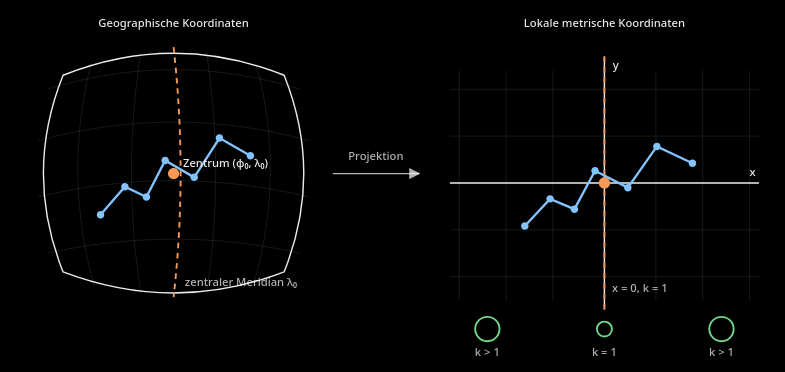
\includegraphics[width=0.5\textwidth]{figures/chapter03/custom_utm_proj.png}
  \caption{Local Transvers Mercator Projection}
  \label{fig:custom-utm}
\end{figure}

Let $c = (\lambda_0, \varphi_0)$ be the center of a trajectory. Then, $\lambda_0$ is used as the central meridian of our Local Transverse Projection, as displayed in \Cref{fig:custom-utm}.
Consequently, $c$ is mapped to the origin of our coordinate system as
\[
\operatorname{lon}_0=\lambda_0,
\qquad
\operatorname{lat}_0=\varphi_0,
\qquad
k_0=1,
\qquad
x_0=y_0=0.
\]

\paragraph{Calculation}
The following formulae describe the LTMP in a simplified manner on a sphere.
For the implementation, one should rather use the ellipsoidal Transverse Mercator transformation on WGS~84 from PROJ.
To calculate the spherical center accurately, we first convert each point $(\lambda_i,\varphi_i)$ to its unit vector representation in three dimensional space:
\[
\mathbf{u}_i= \begin{pmatrix} \cos\varphi_i\cos\lambda_i\\ \cos\varphi_i\sin\lambda_i\\ \sin\varphi_i \end{pmatrix}.
\]
Afterwards, we calculate the averaged vector as 
\[
\bar{\mathbf{u}} = \frac{1}{n}\sum_{i=1}^{n}\mathbf{u}_i = \begin{pmatrix} \bar{x}\\ \bar{y}\\ \bar{z} \end{pmatrix}.
\]
, from which we can extract the geographic coordinates of the center as
\[
\begin{aligned}
    \lambda_0
    &=
    \operatorname{atan2}(\bar{y},\bar{x}), \\
    \varphi_0
    &=
    \operatorname{atan2}
    \left(
        \bar{z},
        \sqrt{\bar{x}^2+\bar{y}^2}
    \right).
\end{aligned}
\]
To project an arbitrary point $(\lambda, \varphi)$ to our LTMP, we first calculate the difference in longitude to our central meridian as
$\Delta\lambda=\lambda-\lambda_0.$
We define $B=\cos(\varphi)\sin(\Delta\lambda)$ as an auxiliary variable, which basically describes the angle-dependent east-west 
distance from the central meridian. The factor $\cos(\varphi)$ accounts for the fact that
longitudes towards the pole correspond to increasingly shorter distances.

Let $R$ denote the radius of the spherical Earth model and $k_0$ the scale foactor along the central meridian. 
The projected coordinates of $(\lambda, \varphi)$ relative to the local origin are then given by
\[
\begin{aligned}
    x
    &=
    \frac{Rk_0}{2}
    \ln\left(\frac{1+B}{1-B}\right), \\
    y
    &=
    Rk_0
    \left[
        \operatorname{atan2}
        \left(
            \tan\varphi,
            \cos\Delta\lambda
        \right)
        -\varphi_0
    \right].
\end{aligned}
\]

It follows from these formulae, that on the central meridian ($\lambda = \lambda_0$), $B = 0$ and therefore $x = 0$. 
Additionally, with $\varphi = \varphi_0$, the second expression evaluates to $y = Rk_0(\varphi - \varphi_0)=0$.
Points west and east of the central meridian receive negative and positive $x$-coordinates, respectively. The factor $Rk_0$ 
converts the angular expressions into metric coordinates.

To quantify the distortion away from the central meridian, we consider the local scale factor \(k\). 
The spherical Transverse Mercator projection can be understood as a Mercator projection applied after rotating the sphere. 
In this rotated coordinate system, \(B\) is the sine of the transverse latitude \(\beta\):

$$
\sin\beta
=
B
=
\cos\varphi\sin\Delta\lambda.
$$

Since the local scale factor of the spherical Mercator projection is \(k_0/\cos\beta\), the scale factor of the spherical Transverse Mercator projection is

$$
k
=
\frac{k_0}{\cos\beta}
=
\frac{k_0}{\sqrt{1-B^2}}.
$$

Close to the central meridian, \(\Delta\lambda\) is small and therefore

$$
B
=
\cos\varphi\sin\Delta\lambda
\approx
\cos\varphi\,\Delta\lambda.
$$

Using the binomial approximation

$$
(1-B^2)^{-1/2}
\approx
1+\frac{B^2}{2},
$$

we obtain

$$
k
\approx
k_0\left(1+\frac{B^2}{2}\right)
\approx
k_0\left(
1+\frac{1}{2}
(\Delta\lambda\cos\varphi)^2\right).
$$

This is the same local scale approximation used for UTM. 
In our LTMP, however, \(k_0=1\) and the central meridian passes through the trajectory center. 
Consequently, the scale is exact along this meridian, and its deviation increases approximately quadratically with the east--west
angular distance from it.

\paragraph{Properties}
The LTMP retains the main properties that make UTM suitable for our workflow. It is conformal, uses metric coordinates, and only distorts lenghts within a predictable,
tolerable scale factor.
However, by placing the central meridian through the trajectory center, scale distortion is minimized for the main area of our trajectories.

Unlike standard UTM CRS, however, an LTMP does not have a standard CRS, which means that projection parameters need to be maintained 
throughout the entire workflow to make inverse reprojections possible.
For compact trajectories located well within a single UTM zone, the numerical difference between UTM and the LTMP is generally 
small. In these cases, the LTMP mainly provides a cleaner and more consistent transformation. 
Its advantages become more relevant for trajectories close to a UTM zone boundary or trajectories with a large east--west extent, and will be evaluated in \Cref{ch:data-environment-bench}.

\subsection{Alternative Projection Candidates}
In addition to UTM and LTMP, other natural projection candidates were examined. Since no projection can preserve angles, distances, and areas simultaneously over a large spatial extent,
 the following projections each focus on preserving a particular geometric property.

\paragraph{Azimuthal Equidistant Projection}
We consider an Azimuthal Equidistant Projection (AEQD) centered on the center coordinate of each trajectory. This projection preserves distances and azimuths from the projection center to every other point. 
Nevertheless, it does not preserve arbitrary pairwise distances, areas, or local angles outside the projection center. Its radial and tangential scales increasingly differ with distance from the center. 
Consequently, isotropic kernels become distorted when applied far from the projection center.

AEQD may be suitable for analyses with a fixed reference point, such as distances from a breeding site, nest, or colony. 
However, it is less suitable for location-independent kernels that should retain the same physical meaning throughout the complete grid.

\paragraph{Lambert Azimuthal Equal-Area Projection}
The Lambert Azimuthal Equal-Area Projection (LAEA) can likewise be centered on each animal's trajectory. It preserves areas exactly, making it a promising candidate for utilization-distribution and home-range calculations. However, it does not preserve distances or local angles. Consequently, local shapes become increasingly distorted with distance from the projection center.

Equal-sized projected cells represent equal areas on the Earth's surface, but their corresponding ground shapes are not identical throughout the grid. 
This can be problematic for random-walk kernels, which rely on locally accurate directions and approximately isotropic cells. 
LAEA is therefore well suited to area-based analyses, but less suitable as the common metric coordinate system for kernel construction and random-walk interpolation.



\paragraph{Web Mercator}
The Web Mercator projection (EPSG:3857) is the standard projection for web maps, including those used by Leaflet, OpenStreetMap, and many tile servers. 
Its common global coordinate system makes it convenient for displaying results such as interpolated trajectories or utilization distributions from multiple animals and study areas on the same map.

In the spherical model underlying Web Mercator, local angles and small shapes are approximately preserved. However, its scale increases with latitude according to
\[
k=\frac{1}{\cos\varphi},
\]
while areas are distorted by approximately \(k^2\).
The scale is therefore correct at the equator but increases rapidly towards the poles.
This causes regions at high latitudes, such as Greenland, to appear disproportionately large compared with regions closer to the equator.

The poles themselves cannot be represented because their projected northing approaches infinity.
Web mapping systems therefore truncate the projection at approximately \(85.05^\circ\) north and south.
For these reasons, Web Mercator is used only for visualization in our pipeline and not for metric distance calculations, kernel construction, or random-walk interpolation.

\section{Grid Discretization}
\label{sec:grid-discretization}

Our random-walk dynamic program does not operate directly on continuous coordinates, but on a discretized grid. Therefore, discretization is required after projecting a trajectory to a metric CRS.

First, we define an animal's bounding box from the coordinate-wise extrema of its projected trajectory:
\[
B
=
(x_{\min},y_{\min},x_{\max},y_{\max}).
\]
Using this bounding box directly would restrict every interpolation to the spatial extent of the observed trajectory. In particular, a movement kernel applied near one of its boundaries could assign probability to positions outside the bounding box. These positions would not be represented by the grid, effectively truncating the kernel and introducing an artificial barrier at the boundary.

We therefore add padding corresponding to \(10\%\) of the bounding-box extent on each side. Let
\[
\begin{aligned}
w &= x_{\max}-x_{\min}, &
h &= y_{\max}-y_{\min},\\
p_x &= 0.1\,w, &
p_y &= 0.1\,h.
\end{aligned}
\]
The padded bounding box is then defined as
\[
\begin{aligned}
B_{\mathrm{pad}}
&=
(E_{\min},N_{\min},E_{\max},N_{\max})\\
&=
\left(
x_{\min}-p_x,\,
y_{\min}-p_y,\,
x_{\max}+p_x,\,
y_{\max}+p_y
\right).
\end{aligned}
\]
Thus, the total width and height are increased to \(120\%\) of their original values.
This additional space allows movement kernels near the observed spatial extremes to extend beyond the trajectory's original bounding box without being immediately truncated.

The parameter \texttt{resolution} defines the number of grid nodes along the longer axis.
The number of nodes along the shorter axis is selected such that the aspect ratio of the padded bounding box is preserved as closely as possible.

\subsection{Projected Coordinates and Grid Nodes}
\label{subsec:projected-coordinates-and-grid-nodes}

For a projected point \((E,N)\), a padded bounding box
\[
(E_{\min},N_{\min},E_{\max},N_{\max}),
\]
and a grid shape \((n_x,n_y)\), the nearest grid node \((i,j)\) is calculated as
\[
\begin{aligned}
i &=
\operatorname{round}
\left(
\frac{E-E_{\min}}{E_{\max}-E_{\min}}
(n_x-1)
\right),\\
j &=
\operatorname{round}
\left(
\frac{N_{\max}-N}{N_{\max}-N_{\min}}
(n_y-1)
\right).
\end{aligned}
\]
Here, \(i\) increases from west to east, while \(j\) increases from north to south to match the row ordering of the grid array.

The corresponding projected coordinates of a grid node are
\[
\begin{aligned}
E' &=
E_{\min}
+
\frac{i}{n_x-1}
(E_{\max}-E_{\min}),\\
N' &=
N_{\max}
-
\frac{j}{n_y-1}
(N_{\max}-N_{\min}).
\end{aligned}
\]
If geographic coordinates are required, \((E',N')\) is subsequently transformed back using the inverse UTM, UPS, or LTMP transformation.

For non-degenerate axes with \(n_x,n_y>1\), the projected spacing between neighbouring grid nodes is
\[
\Delta E
=
\frac{E_{\max}-E_{\min}}{n_x-1},
\qquad
\Delta N
=
\frac{N_{\max}-N_{\min}}{n_y-1}.
\]
Since each point is mapped to its nearest grid node, the projected quantization error is bounded by half of the cell diagonal:
\[
\epsilon
\leq
\frac{1}{2}
\sqrt{\Delta E^2+\Delta N^2}.
\]
Consequently, the selected grid resolution directly affects the discretization error, independently of the distortion introduced by the map projection.
This relationship is examined in the following subsection.


\section{Projection Benchmark}
\label{sec:projection-benchmark}
Thus far, several projections have been presented.
In this section, their suitability for local step calculations (e.g., distance, velocity), kernel generation and interpolations on a regular grid will be examined.
In this context, projection distortion and grid discretization errors are inspected separately.
Furthermore, we check whether spatial windowing helps to reduce the high deviations caused by single projections for long-range studies.

We measure the projection- and discretization error using the shortest ellipsoidal geodesics on WGS~84 between original points and mapped points.

\subsection{Benchmark Datasets}
\label{subsec:projection-benchmark-datasets}
To cover a range of spatial conditions, we select four diverse studies: The first two are the Slovenia Bears and Siberia Rubythroat studies, detailed in \Cref{ch:datasets}.
The Bears study is representative for localized terrestrial trajectories
that span a few kilometers at most, while the Rubythroat study represents migration studies of airborne or marine animals,
spanning multiple UTM zones and a large extent of longitude and latitude.
The third dataset is a wide-ranging Arctic fox tracking study.
It is intended to stress test our local Mercator projections near the poles, while remaining within the regular UTM latitude domain.
Its trajectories are positioned at a high latitude with a wide longitude range of around $56\circ$.
It is therefore used to examine the behavior of UTM/UPS and LTMP for extensive high-latitude trajectories.
The final study is a synthetic polar track, north of the UTM latitude domain of $84\circ$.
It crosses the Internation Date Line (IDL) and circles the pole multiple times.
This extreme case is intended as a numerical stress test to compare UPS with local projections rather than for analyzing realistic trajectories.

\begin{table}[htbp]
    \centering
    \caption{Datasets used for the projection benchmark.}
    \label{tab:projection-benchmark-datasets}
    \begin{tabular}{llll}
        \toprule
        Dataset & Selected individual & Fixes & Purpose \\
        \midrule
        Slovenia bears
            & \texttt{ancka}
            & 351
            & Compact regional trajectory \\
        Siberian rubythroat
            & \texttt{X49996}
            & 40
            & Long-range migration \\
        Arctic fox
            & \texttt{MMRV}
            & 1502
            & High-latitude, wide-ranging movement \\
        Synthetic polar track
            & ---
            & 72
            & Polar and antimeridian stress case \\
        \bottomrule
    \end{tabular}
\end{table}

\subsection{Methodology}
\label{subsec:projection-benchmark-methodology}
The following metrics are used to quantify the distortion errors of the respective projections.

\paragraph{Distance fidelity}
\label{par:Dist-fid}
To benchmark length preservation, we compare the Euclidean distance ($d_{p,k}$) in the projected CRS with the ellipsoidal WGS~84
geodesic distance ($d_{g,k}$), which represents the shortest distance between the
two points on the Earth's curved surface.

\[
d_{g,k}=d_{geo}(p_k,q_k),
\qquad
d_{p,k}
=
\sqrt{
    (E_{q,k}-E_{p,k})^2
    +
    (N_{q,k}-N_{p,k})^2
}.
\]

The absolute percentage error of the \(k\)-th point pair is

\[
u_k
=
100
\frac{|d_{p,k}-d_{g,k}|}{d_{g,k}}.
\]

The Mean Absolute Percentage Error (MAPE) is obtained by averaging these
errors over all \(m\) evaluated point pairs:

\[
\operatorname{MAPE}
=
\bar{u}
=
\frac{1}{m}
\sum_{k=1}^{m} u_k.
\]

Additionally, we report the 95th percentile of the absolute relative
distance error,

\[
u_{95}
=
Q_{0.95}(u_1,\ldots,u_m),
\]

which is the value below which approximately 95\% of the observed
percentage errors fall.

For this distance fidelity benchmark, the deviations of consecutive (non-identical) point pairs, as well as random pairs within the same trajectory are averaged.
The test with consecutive pairs is relevant for the calculation of segmentation features like distance and turn angle and velocities for kernel generation.
Random pairs are evaluated to explore the distortion across the entire spatial extent of a trajectory, which is relevant for utilization distributions and visualizations of complete tracks.

\paragraph{Local scale and directional distortion}
To quantify local shape and length distortion, we calculate the following Tissot factors for every fix.
Consider an infinitesimally small neighborhood around each fixed point, for example, a tiny circle on the Earth's surface.
Through projection, this circle becomes an ellipse with semi-axes \(a_i\) and \(b_i\):
These Tissot semi-axes $a_i$ and $b_i$ denote the maximum and minimum scale distortions in the i'th point of a trajectory, respectively.

Consequently,
  \[
  s_i=100\max(|a_i-1|,|b_i-1|)
  \]
measures the largest local scale distortion, while the Tissot-anisotropy
  \[
  A_i=\frac{a_i}{b_i}
  \]
measures the local shape or directional distortion.
For example, a projection with $a_i=b_i=1.4$ scales lengths by $s_i=40\%$, while remaining shape preserving, as $A_i=1$.

In our benchmark, we calculate the 95th percentile of the local scale factors $s_i$, as well as the maximum and average Tissot-anisotropies $A_{mean}$ and $A_{\max}$.

\paragraph{Grid discretization error}
To quantify the error induced by rasterization to our dynamic program grid, we convert each fix to its metric CRS,
round each coordinate to the next regular grid node, and transform back to WGS~84.
The resulting geodetic displacement error between the original ($p_i$) and reprojected ($P^{-1}\!\left(S(P(p_i))\right)$) fix is

\[
g_i
=
d_g
\left(
    p_i,
    P^{-1}\!\left(S(P(p_i))\right)
\right),
\]
where $S$ denotes the mapping of a point to the closest grid node.

At first, we examine how the different projections perform under the same reference resolution of $R = 1024$ using the 95th percentile, minimum and maximum values of $g_i$.
Additionally, we isolate the discretization error with regard to varying resolutions.
A resolution sweep with
\[
    R\in
    \{32,64,128,256,512,1024,2048\}.
\]
is supposed to show to what extent error decreases with increasing resolution for the different kinds of studies.
The projected half-cell diagonal from \Cref{subsec:projected-coordinates-and-grid-nodes} is also used as a theoretical reference.

\subsection{Windowing for Long-Range Trajectories}
\label{subsec:projection-windowing-method}
A long-range trajectory spanning multiple thousands of kilometers practically results in large grid cells, as the grid resolution cannot
be arbitrarily increased due to computational limitations. Large grid cells are problematic for a multitude of reasons. Firstly, physical kernels
may collaps to single cells when rasterized to the DP grid.
Secondly, fixes close to each other, for example in foraging stages, would be projected to the same grid cell and only travelling states can be interpolated. Finally, 
large cell diameters lead to higher discretization errors according to \Cref{form:grid-error}. 

Besides, points far from the projection center inevitably display large scale and shape distortions.
Long-range trajectories are therefore broken down into spatially limited windows.
For this, we use the following greedy partitioning procedure:
\begin{algorithm}[H]
\caption{Greedy-Partitioning with disc criterium}
\begin{algorithmic}[1]
\Require Trajectory $\tau = (p_1,\dots,p_n)$, radius $r = 50\,\mathrm{km}$
\Ensure Windows $W_1,\dots,W_k$ satisfying $C$ 
\State $i \gets 1$; \; $\mathcal{W} \gets \emptyset$
\While{$i < n$}
  \State $j \gets i + 1$
  \While{$j \le n$ \textbf{and} $d_{\mathrm{geo}}(p_i, p_j) \le r$}
    \Comment{$C(i,j)$}
    \State $j \gets j + 1$
  \EndWhile
  \State $j \gets j - 1$
    \Comment{largest $j$ with $C(i,j)$}
  \If{$j = i$}
    \State $j \gets i + 1$
      \Comment{Sprung $> r$: Single step as its own Window}
  \EndIf
  \State $\mathcal{W} \gets \mathcal{W} \cup \{(i,j)\}$
  \State $i \gets j$
    \Comment{Cut bei $j$, next window starts with endpoint}
\EndWhile
\State \Return $\mathcal{W}$
\end{algorithmic}
\label{alg:windowing-algorithm}
\end{algorithm}
The partitioning criterion $C(i, j)$ is defined such that it evaluates to true, 
if and only if all fixes $p_i,\dots,p_j$ lie inside the disc of radius $r=50\,\mathrm{km}$ around the anchor $p_i$,
meaning $d_{\mathrm{geo}}(p_i, p_k) \le r$ for all $k \in [i,j]$. $C$ is \emph{decreasing monotone}: 
If $C(i,j)=1$, then also $C(i',j')=1$ for each $[i',j'] \subseteq [i,j]$ with the same anchor $p_i$, 
making the greedy partitioning algorithm permissible.
As a consequence, the diameter of each window is at most $100 \,\mathrm{km}$.
Furthermore, the windows overlap in exactly one fix (see line 12) so that each step lies entirely in one window.

To evaluate the gain in precision from our windowing procedure, we compare the trajectories' MAPEs with windowing with the MAPEs using a single bounding box per trajectory using 
\[
G = 100 \left(1-\frac{M_{\mathrm{window}}}{M_{\mathrm{full}}}\right)\%.
\]
Here, $G$ denotes the relative error-reduction caused by windowing. 
Additionally, we report the maximum number of fixes in a single cell. Many fixes sharing a cell results in loss of information, as spatially close fixes are not interpolated and reprojected to the same point in geodesic coordinates. 
Ideally, they are only permissible for resting stages.
For this part of the experiments we use our two long-range studies Siberian Rubythroat and Arctic Fox.



\subsection{Results}
\label{subsec:projection-benchmark-results}
\subsubsection{Distance fidelity}
The plots in \Cref{fig:dist-fidelity} show a comparison of length distortion, expressed as the mean absolute percentage error, between the different projection types per study.
\label{subsubsec:dist-fidelity}
\begin{figure}[h]
        \centering
        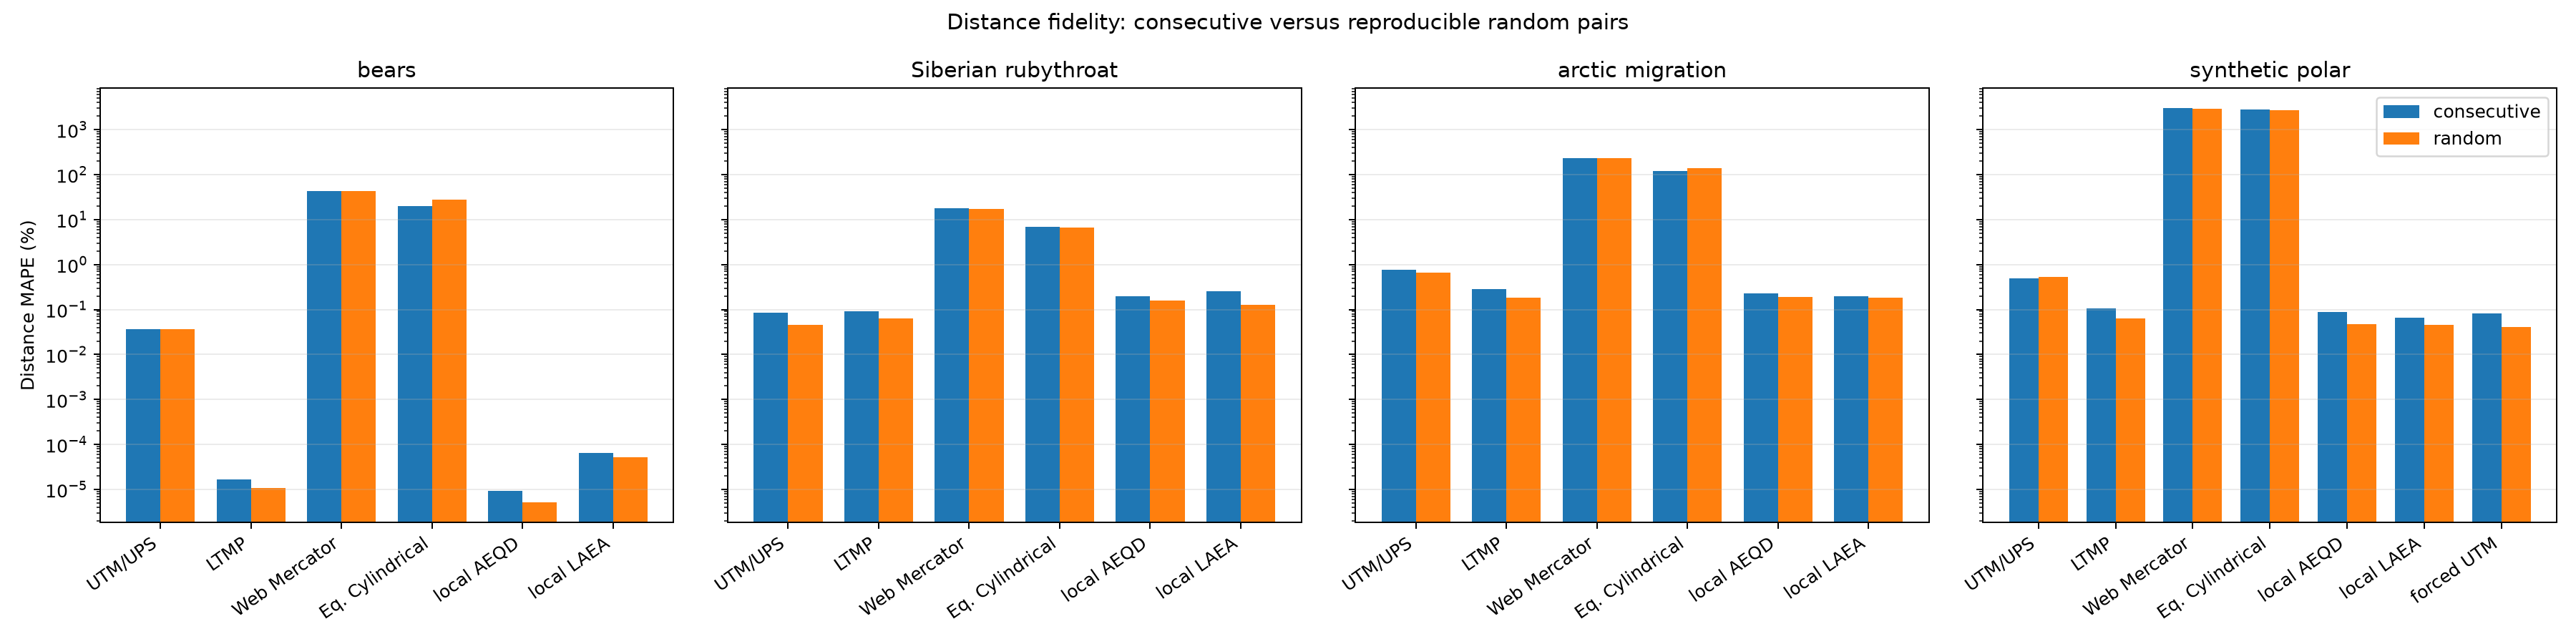
\includegraphics[width=\textwidth]{figures/chapter03/bench/distance_fidelity}
        \caption{}
        \label{fig:dist-fidelity}
\end{figure}
As expected, the Web Mercator projection exhibits the greatest scale distortion across all studies.
The remaining projections have relatively low percentage errors, never exceeding 1\%, and the best projection depends on the dataset.
Notably, in the Slovenia Bears study, LTMP and AEQD exhibit significantly lower errors than UTM and LAEA.
This can be explained by the study's low range, which results in a relatively high proximity to the projection center compared to UTM.
Whether consecutive or random point pairs are examined, does not have any influence on the general trend.
\subsubsection{Local scale and directional distortion}
\Cref{fig:anisotropy} displays the comparisons of local length and shape distortion, using the 95th percentile of the largest local scale distortion metric, $s_i$, and the Tissot anisotropy, $A_i$.
\label{subsubsec:anisotropy}
\begin{figure}[h]
        \centering
        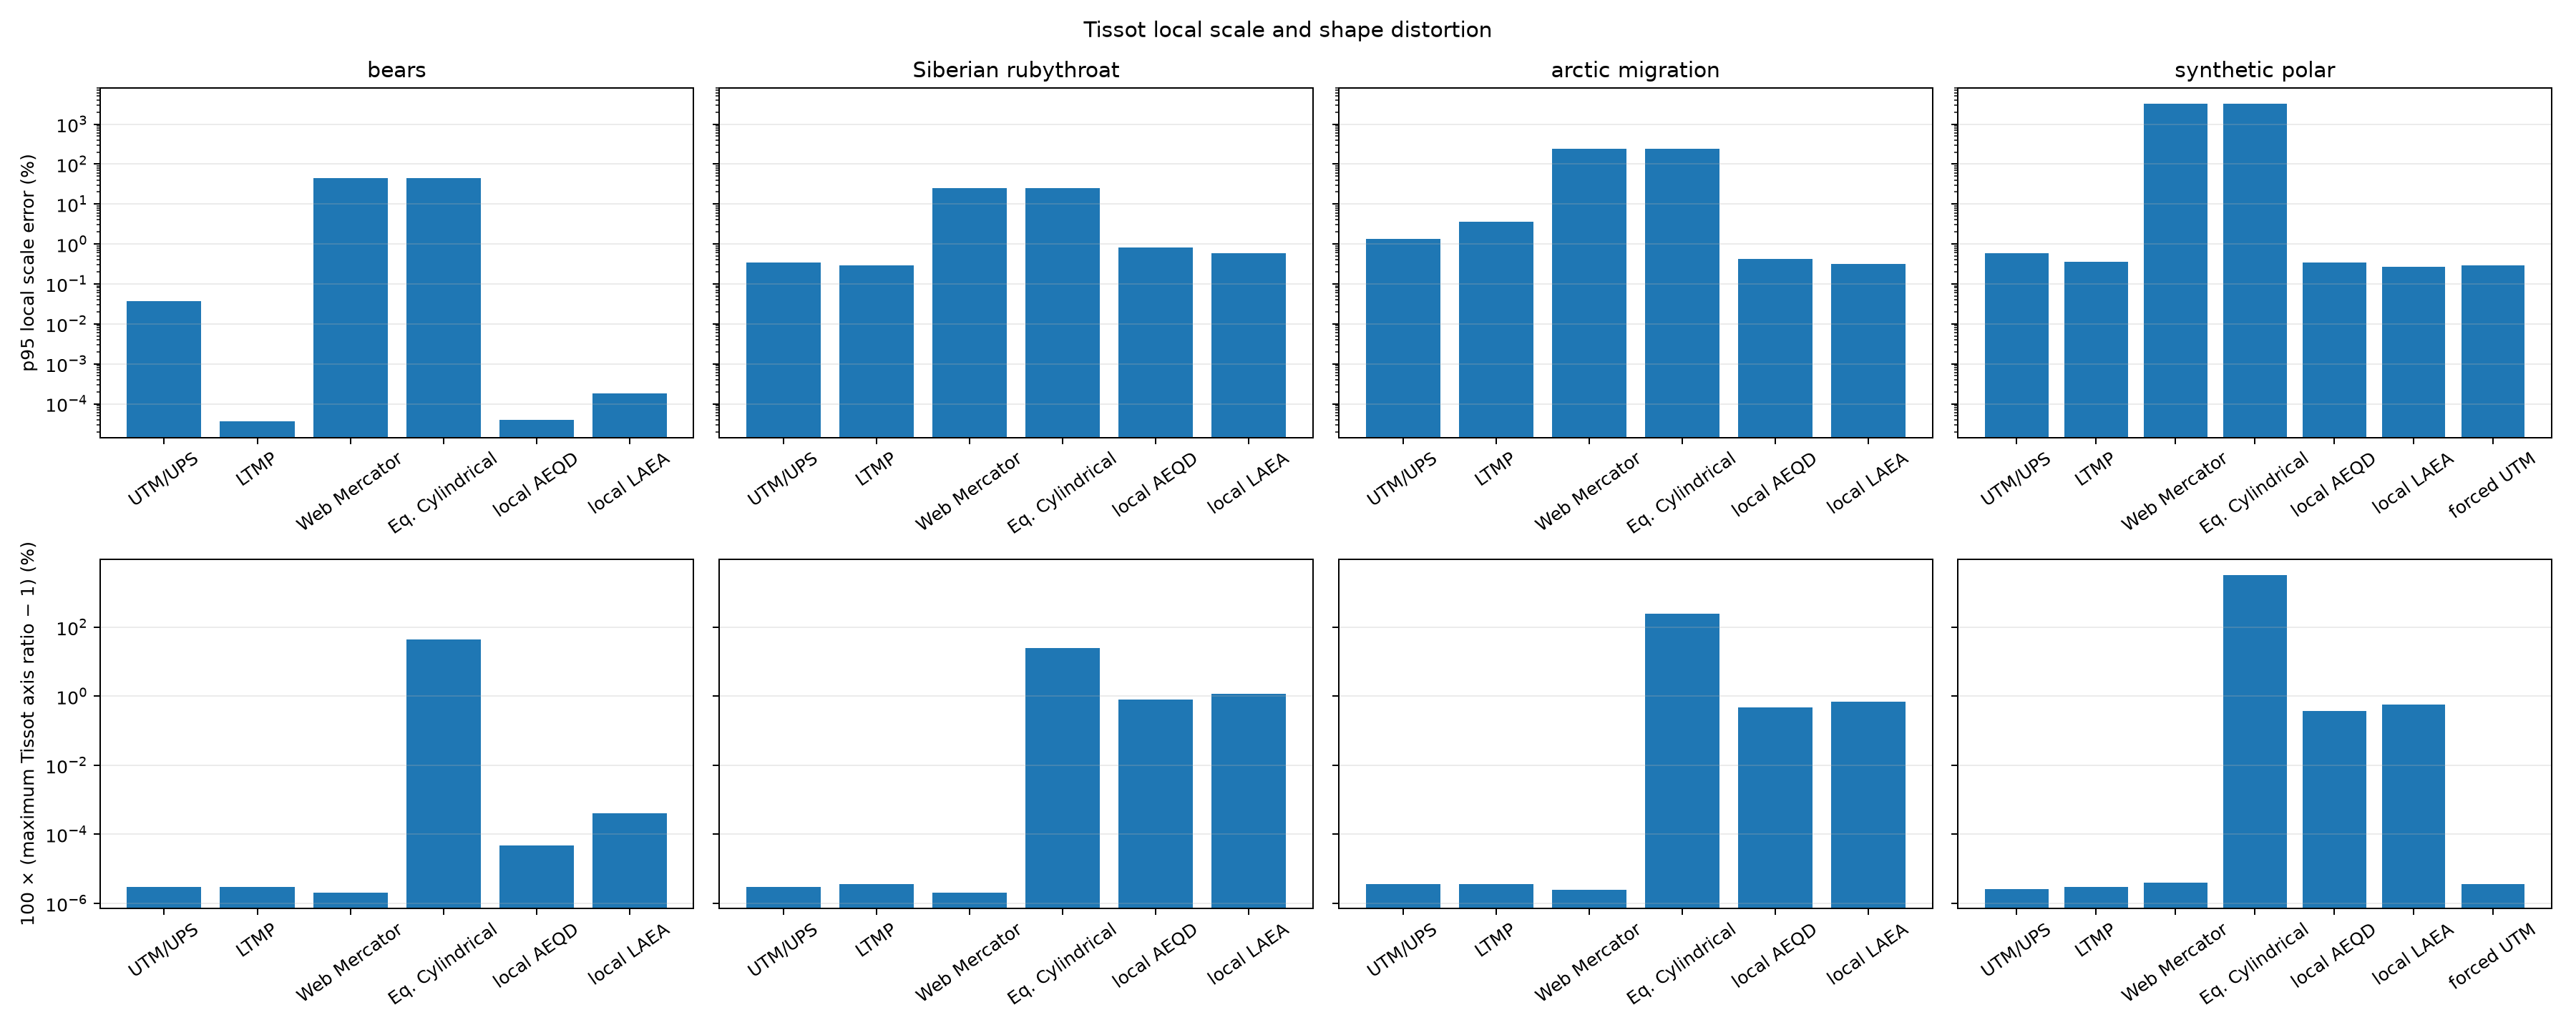
\includegraphics[width=\textwidth]{figures/chapter03/bench/local_scale_and_anisotropy}
        \caption{}
        \label{fig:anisotropy}
\end{figure}
The results for scale distortion show a similar overall pattern to the results from \Cref{fig:dist-fidelity}.
Web Mercator exhibits the highest scale error across all studies.
UTM, LTMP, and both Azimuthal projections result in much lower scale error, with their ordering depending on the dataset.
Once again, LTMP and AEQD achieve comparatively much lower error rates in the locally confined bears study.


In terms of shape distortion, both UTM/UPS and LTMP demonstrate Tissot's anisotropy close to unity, which is consistent with their conformality and the preservation of local angles.
In contrast, the two azimuthal projections demonstrate directional distortion.
AEQD preserves distances from the projection centre, while LAEA preserves area; however, neither projection generally preserves local angles.
The Web Mercator projection also shows very low anisotropy in this benchmark, but since it has the worst scale distortion of all the projections compared,
it is unsuitable for the metric computations considered here

\subsubsection{Grid discretization error}
\label{subsubsec:grid-discretization-error}
The plot in \Cref{fig:error-res} depicts the 95th percentile round-trip error $G_{95}$, primarily caused by grid-discretization, for our study-set using either UTM/UPS or LTMP.

\begin{figure}[h]
    \centering
    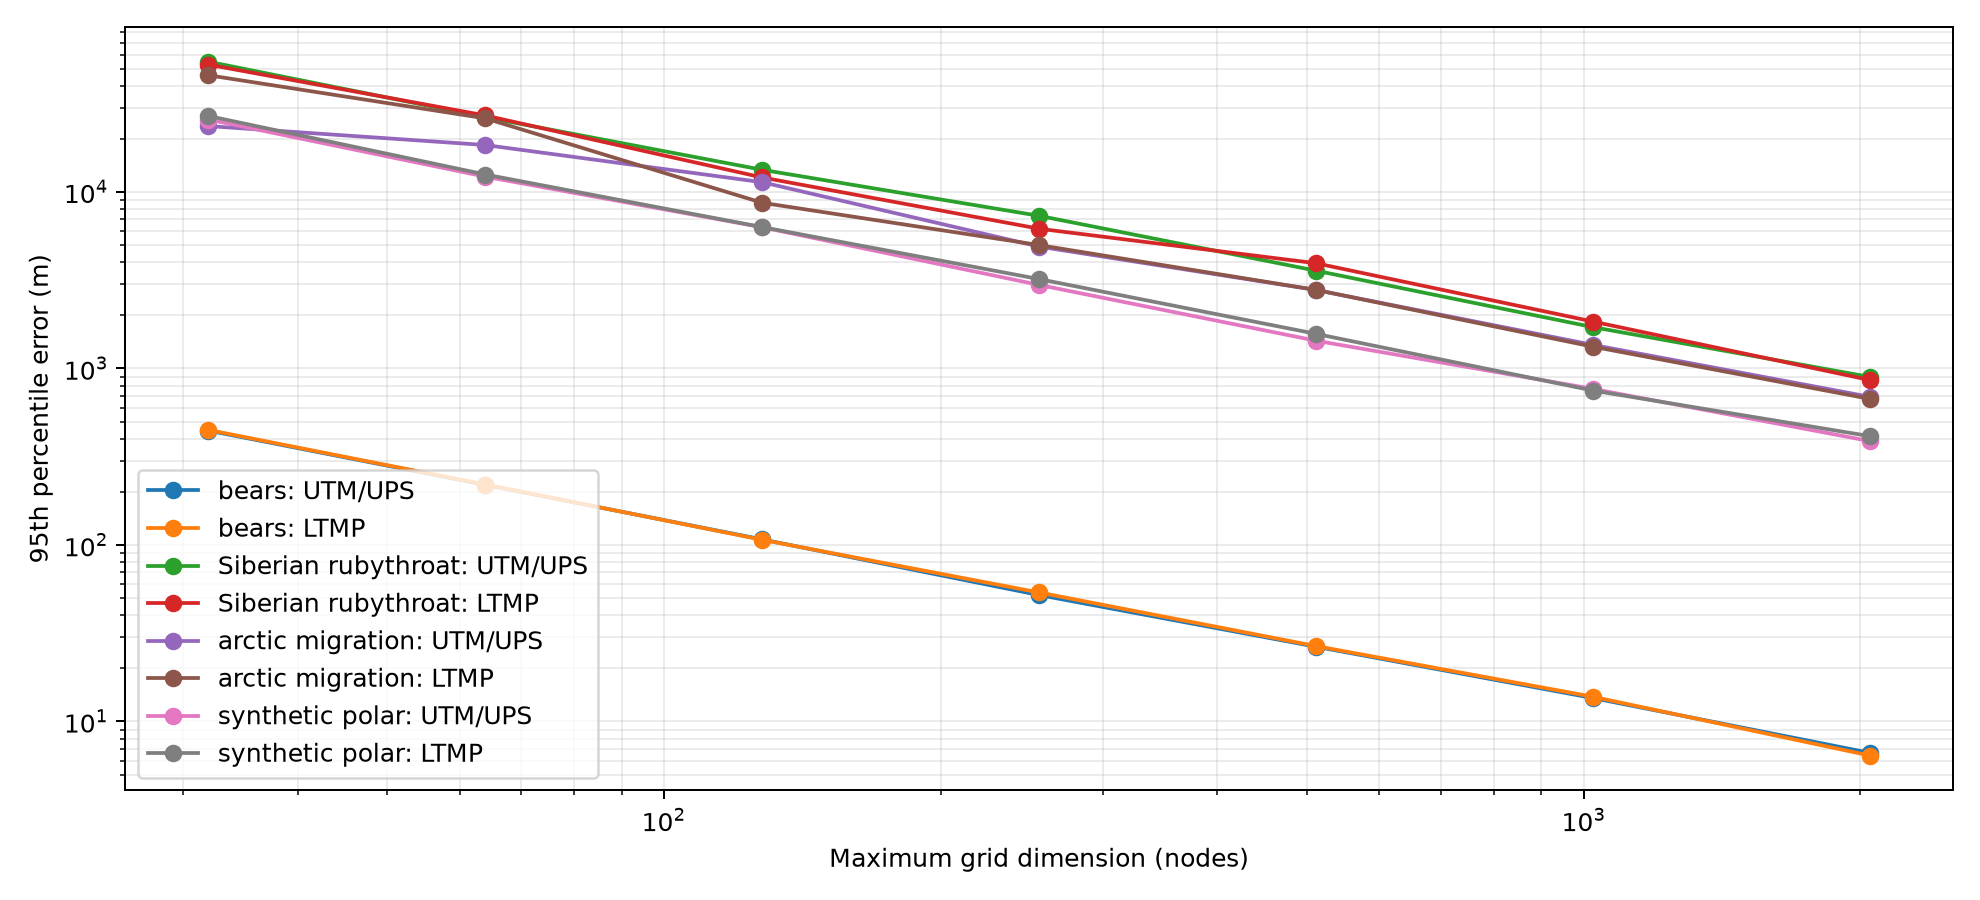
\includegraphics[width=\textwidth]{figures/chapter03/bench/error_by_resolution}
    \caption{}
    \label{fig:error-res}
\end{figure}

It is evident that the discretization error decreases with increasing resolution, as the projected quantization error $\epsilon$ decreases with smaller cell sizes.
Using either UTM/UPS or LTMP does not affect the general trend.
Overall, long-range studies still exhibit large deviations of approximately $1.3-1.8 \mathrm{ km}$, even at high resolutions such as 1024.
In cases like these, the windowing procedure from \Cref{alg:windowing-algorithm} allows for a more detailed spatial representation per window while maintaining the same grid resolution
and comparable computational cost per interpolation.

\subsubsection{Windowing for Long-Range Trajectories}
\label{subsubsec:bench-windowing}
\Cref{fig:windowing-comp} illustrates the comparison of the 95th percentile geodesic grid displacement $Q_{95}$ and the distance
preservation metric MAPE for both single window projections and independent local windows with a fixed radius of $50 \mathrm{km}$ and grid resolution of 1024 for two long-range studies.

\begin{figure}[h]
    \centering
    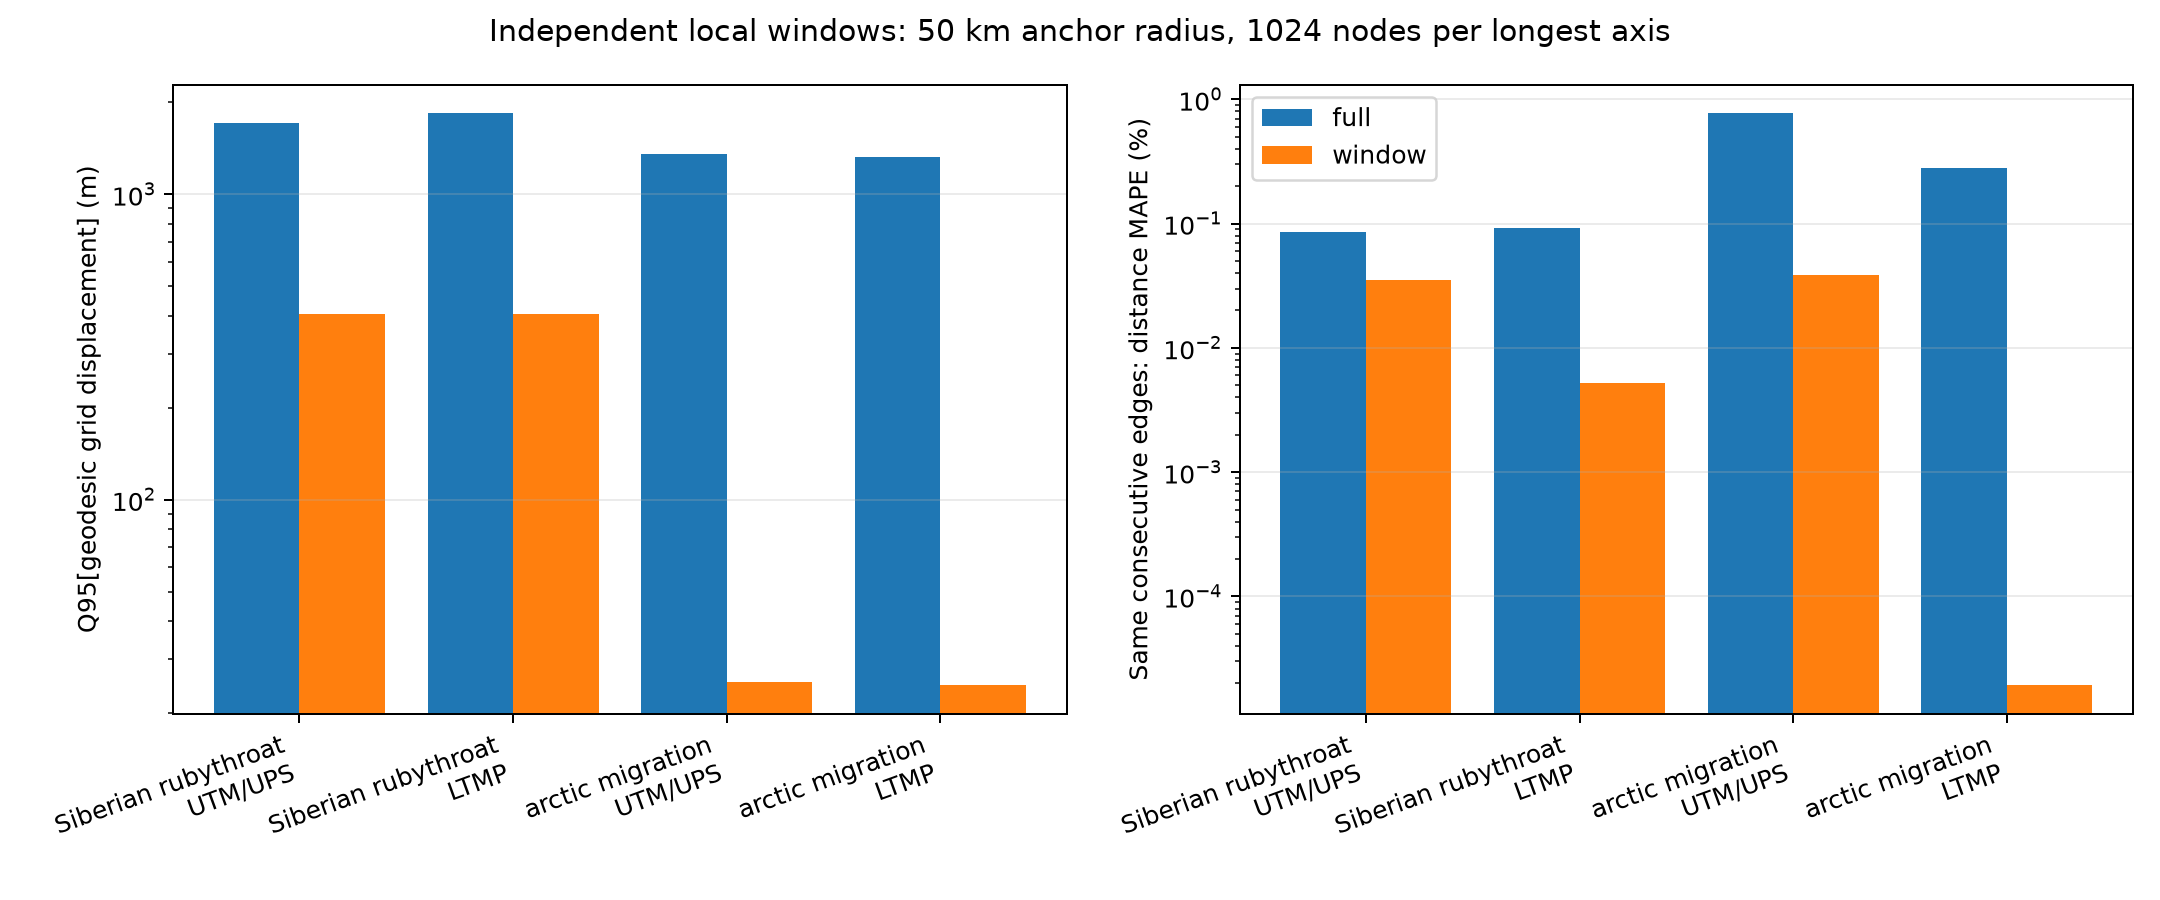
\includegraphics[width=\textwidth]{figures/chapter03/bench/windowing_comparison}
    \caption{}
    \label{fig:windowing-comp}
\end{figure}

Regarding geodesic grid displacement, the $Q_{95}$ error decreased by $76-78\%$ for the rubythroat migration study and $98\%$ for the arctic fox study.
Here, the difference between UTM/UPS and LTMP is negligible.
Windowing yields similar improvements in MAPE, with error decreasing by up to $94.4\%$ for the rubythroat study and $99.993\%$ for the arctic fox study.
Compared to UTM, LTMP yields considerably lower distance errors, particularly in the Arctic fox study.

The Arctic fox trajectory benefits more from windowing because oversized jumps are relatively rare and much shorter than those in the rubythroat trajectory.
Consequently, large windows affect a smaller proportion of fixes and have less influence on the pooled 95th-percentile grid displacement.
In contrast, the sparsely sampled rubythroat trajectory contains several steps of over 1000 km, resulting in large windows with significant remaining discretization error.


\subsubsection{Benchmark Conclusion}
\label{subsubsec:bench-conclusion}
In terms of length and shape preservation, UTM and LTMP are the most suitable projections. 
While azimuthal equal-distance/area projections perform comparatively well in scale distortion metrics, their lack of conformality becomes evident when examining local shape preservation using Tissot's anisotropy. 
This renders AEQD and LAEA unsuitable for transition kernel calculations. 
In general, Web Mercator should be reserved for visualizations because it performed the worst in the distance fidelity and local scale distortion benchmarks.

Grid discretization plays a more important role in preventing large displacement errors when converting from one CRS to another, than the choice of projection. 
Increasing the grid resolution significantly decreases displacement error for every study examined.
Furthermore, windowing for long-range trajectories helps reduce displacement error drastically, especially in our study of the Arctic Fox polar region.

In conclusion, UTM or LTMP is recommended for the entire workflow and for any kind of dataset.
Windowing should always be performed for long-range trajectories to reduce displacement errors and other undesirable effects caused by large grid cells (e.g., many close original fixes collapsing into one grid cell).
Windowing can also reduce computational costs because multiple low-resolution windows are more efficient (in terms of time and space) than one large window for random walk calculations, while offering a more detailed spatial representation. 
In this context, LTMP is a more natural choice than UTM, as the projection centers coincide with each window's center, and LTMP also performs slightly better.

\section{Terrain Annotation}
\label{sec:terrain-annotation}
The final step of our first module is to annotate our trajectory collection with environmental information.
More precisely, each observed trajectory point is assigned a terrain class, such as LAND/WATER, for studies with a large spatial extent (e.g., airborne or marine animals),
or the specific type of land for localized (terrestrial) trajectories.

\subsection{Range Type: Local}
\label{subsec:range-local}
This setting \texttt{RangeType.LOCAL} uses ESA WorldCover to obtain detailed land-cover information at a resolution of $10\,\mathrm{m}$.
The local land-cover maps are provided through Microsoft's Planetary Computer STAC API
\footnote{\url{https://planetarycomputer.microsoft.com/api/stac/v1/collections/esa-worldcover}}
in the form of GeoTIFFs in EPSG:4326.

For every animal, the application performs the following steps:
\begin{enumerate}
    \item The trajectory is transformed to EPSG:4326 (if provided in a different CRS)
    \item Its geographic bounding box is determined as
    \[
        (\lambda_{\min},\varphi_{\min},
        \lambda_{\max},\varphi_{\max}).
    \]
    \item A padding of $10\%$ is added on each side.
    Minimum padding of $0.0001^\circ$ prevents degenerate requests for trajectories with a tiny extent.
    \item The STAC collection \texttt{esa-worldcover} is searched using the padded bounding box.
    \item The returned asset URLs are signed using \texttt{planetary\_computer.sign\_inplace}.
    \item The categorical \texttt{map} asset is selected and clipped to the requested extent.
\end{enumerate}

The WorldCover raster distinguishes the classes and colors enumerated in the \Cref{tab:worldcover-classes}.

\begin{table}[htbp]
\centering
\caption{ESA WorldCover land-cover classes and their standard display colors.}
\label{tab:worldcover-classes}
\begin{tabular}{rll}
\toprule
Code & Class & Color \\
\midrule
10  & Tree cover               & \colorswatch{006400}\quad\texttt{\#006400} \\
20  & Shrubland                & \colorswatch{FFBB22}\quad\texttt{\#FFBB22} \\
30  & Grassland                & \colorswatch{FFFF4C}\quad\texttt{\#FFFF4C} \\
40  & Cropland                 & \colorswatch{F096FF}\quad\texttt{\#F096FF} \\
50  & Built-up                 & \colorswatch{FA0000}\quad\texttt{\#FA0000} \\
60  & Bare or sparse vegetation & \colorswatch{B4B4B4}\quad\texttt{\#B4B4B4} \\
70  & Snow and ice             & \colorswatch{F0F0F0}\quad\texttt{\#F0F0F0} \\
80  & Permanent water bodies   & \colorswatch{0064C8}\quad\texttt{\#0064C8} \\
90  & Herbaceous wetland       & \colorswatch{0096A0}\quad\texttt{\#0096A0} \\
95  & Mangroves                & \colorswatch{00CF75}\quad\texttt{\#00CF75} \\
100 & Moss and lichen          & \colorswatch{FAE6A0}\quad\texttt{\#FAE6A0} \\
\bottomrule
\end{tabular}
\end{table}

The annotations performed at this stage of the pipeline can later be used to train terrain-specific transition kernels.
These kernels can then be used to identify differences in an animal's local movement patterns depending on the terrain.
Furthermore, thanks to the high resolution of GeoTIFF, we can use the same API to modify transition probabilities within a single displacement by enumerating the terrain patches crossed in that step.
This procedure is detailed in \Cref{chap:kernels}.

\subsection{Range Type: Long Range}
\label{subsec:long-range}
One limitation of the Planetary Computer STAC API is that the provided GeoTIFFs are restricted to interior land and coastal regions, and are therefore too small in extent for studies of bird migration or marine animals.
Subdividing the query area into manageable patches and combining them would be too elaborate and costly in terms of API rate limits.
Furthermore, for these two types of study, a detailed breakdown of the terrain crossed would be excessive.
It is usually sufficient to determine whether the animal is in or above water or land.
The setting \texttt{RangeType.LONG} therefore uses the packaged Natural Earth land dataset.%
\footnote{\url{https://www.naturalearthdata.com/downloads/10m-physical-vectors/10m-land/}}

The dataset consists of global land polygons, including major islands, at a cartographic scale of $1{:}10,000,000$.
The shapefile is distributed with the application and does not require access to an external API\@.
Analogous to the local range type, the polygon set is queried with each trajectory's padded bounding box.
The selected polygons are rasterized to a GeoTIFF file, such that (for compatibility reasons with the local range type),
land is mapped from code 1 to 10 (\texttt{TREE\_COVER}) and water is mapped from 0 to 80 (\texttt{PERMANENT\_WATER}).
After that, both modes use the same processing steps to achieve land-cover annotation.

\subsection{Raster Reprojection and Annotation}
\label{subsec:raster-reprojection-and-annotation}
The acquired or generated terrain raster is reprojected to the user-selected, locally metric coordinate reference system (CRS).
Then, the projected GeoTIFF is subsampled or supersampled to the regular grid dimensions using nearest-neighbor interpolation, as described in \Cref{sec:grid-discretization}.
The result is a terrain grid that matches the resolution of the dynamic program array and contains the desired land cover information.
Subsequently, each location is queried from its corresponding transformed terrain raster.
Finally, grid indices, terrain codes, and readable descriptors (see \Cref{tab:worldcover-classes}) are added to each record of each trajectory.


The complete terrain-annotation procedure can be summarized as follows:

\begin{algorithm}[htbp]
\caption{Per-animal terrain annotation}
\label{alg}
\begin{algorithmic}[1]
\Require trajectory collection \(T\), range type \(r\), projection \(p\), resolution \(q\)
\Ensure annotated collection, and per-animal terrain artifacts

\State \(T' \gets\) copy of \(T\)

\ForAll{animal trajectories \(t\) in \(T'\)}
\State Validate the CRS and point coordinates
\State Transform \(t\) to WGS~84
\State Determine and pad the geographic acquisition extent
\State Reject unsupported extents crossing the antimeridian

\State Select UTM/UPS or a trajectory-centred LTMP as the grid CRS
\State Project the trajectory into the grid CRS
\State Construct the regular grid according to \Cref{sec:grid-discretization}
\State Assign every observed point to its nearest grid node

\If{\(r=\texttt{LOCAL}\)}
    \State Query the ESA WorldCover STAC collection
    \State Select and clip the signed categorical \texttt{map} asset
\Else
    \State Load the packaged Natural Earth land polygons
    \State Rasterize the selected polygons as land and water
\EndIf

\State Reproject the terrain raster to local UTM/UPS
\State Use nearest-neighbor resampling to preserve category codes

\State Transform the DP-grid nodes into the raster CRS
\State Sample the terrain raster at every grid node
\State Transform and sample the original trajectory points

\If{\(r=\texttt{LONG\_RANGE}\)}
    \State Map the binary classes to \(10=\text{Land}\) and \(80=\text{Water}\)
\EndIf

\State Append terrain classes, names, grid indices, and projected coordinates
\State Save the per-animal terrain TIFF and terrain grid for the ensuing pipeline steps
\EndFor

\State \Return \(T'\)
\end{algorithmic}
\end{algorithm}


\section{MoveApp}
\label{sec:env-moveapp}
